\section{Results} \label{results}

EvoSuite was run on 12 different Java classes.
The results regarding branch coverage of each class are reported in Table \ref{classescov}.
In the following sections, the cyclomatic complexity of the CUT is reported respectively with corresponding branch coverage and test code readability. 
The correlations between the results are calculated according to Pearson's correlation coefficient formula \cite{DEKKING2005}:
\begin{center}
r = 
$
\frac{\displaystyle\sum_{i}(x_i - \bar{x})(y_i - \bar{y})}
{\sqrt[]{\displaystyle\sum_{i}(x_i - \bar{x})^2}\sqrt{\displaystyle\sum_{i}(y_i - \bar{y})^2}}
$
\end{center}

{\setlength{\extrarowheight}{1ex}
\begin{table}[tbp]
\begin{center}
\begin{tabular}{ m{8cm} c }
\hline 
Class & Coverage \\ [0.5ex]
\hline
PrimeChecker.isPrime & 83\% \\ [0.5ex] 
IntStack & 100\%  \\ [0.5ex]
EnglishNumberToWords & 73\%  \\ [0.5ex]
ColourPicker & 85\% \\ [0.5ex]
org.joda.time.chrono.ISOChronology & 83\%  \\ [0.5ex]
org.joda.time.DateTimeUtils & 56\% \\ [0.5ex]
com.google.common.base.Absent & 50\%\\ [0.5ex]
com.google.common.base.Optional & 33\% \\ [0.5ex]
com.google.common.base.Present & 100\% \\ [0.5ex]
com.google.common.base.Strings & 84\% \\ [0.5ex]
com.google.common.math.IntMath & 81\% \\ [0.5ex]
com.google.common.graph.ImmutableGraph & 100\% \\ [0.5ex]
\hline
\end{tabular}
\end{center}
\caption{For each class, the table reports the branch coverage achieved by the EvoSuite framework.}
\label{classescov}
\end{table}
}

\subsection{Cyclomatic Complexity and Code Coverage}

The results for the cyclomatic complexity of the CUT and branch coverage are reported in Table \ref{cyccov}.
With Pearson's formula, the resulting correlation coefficient is 0.1753. 
Despite this result being positive, the relationship between cyclomatic complexity and branch coverage is weak.
This value is too close to 0 to establish any rule on the influence of code complexity on code coverage. 

Although the number of classes being relatively low, the types of classes were variate. 
From data classes to single-method classes with high complexity, it seems these characteristics had no influence on the total coverage achieved by EvoSuite.
It is possible assume that \textbf{cyclomatic complexity of the CUT has no influence on the total branch coverage reached}, but given the small dataset of classes, it is unwise to draw final conclusions. 

{\setlength{\extrarowheight}{1ex}
\begin{table}[tbp]
\begin{center}
\begin{tabular}{ m{6cm} c c }
\hline 
Method & Cyclomatic Complexity & Coverage \\ [0.5ex]
\hline
PrimeChecker.isPrime & 6 & 83\% \\ [0.5ex] 
IntStack & 2.143 & 100\%  \\ [0.5ex]
EnglishNumberToWords & 4.667 & 73\%  \\ [0.5ex]
ColourPicker & 18 & 85\% \\ [0.5ex]
org.joda.time.chrono.ISOChronology & 1.8 & 83\%  \\ [0.5ex]
org.joda.time.DateTimeUtils & 2.226 & 56\% \\ [0.5ex]
com.google.common.base.Absent & 1.071 & 50\%\\ [0.5ex]
com.google.common.base.Optional & 1.222 & 33\% \\ [0.5ex]
com.google.common.base.Present & 1.167 & 100\% \\ [0.5ex]
com.google.common.base.Strings & 3.6 & 84\% \\ [0.5ex]
com.google.common.math.IntMath & 6.6 & 81\% \\ [0.5ex]
com.google.common.graph.ImmutableGraph & 1.727 & 100\% \\ [0.5ex]
\hline
\multicolumn{2}{m{6cm}}{Correlation} & 0.1753 \\ [0.5ex]
\hline
\end{tabular}
\end{center}
\caption{For each class, the table reports the average cyclomatic complexity of that class and the total branch coverage achieved by EvoSuite.}
\label{cyccov}
\end{table}
}

\subsection{Cyclomatic Complexity and Test Readability}

The results for the cyclomatic complexity of the CUT and average test readability score given by the team members are reported in Table \ref{cycread}.
With Pearson's formula, the resulting correlation coefficient is 0.3044.
This coefficient is weak, which shows little relationship between the results.

The ColourPicker class was orchestrated to hold a very high cyclomatic complexity, but the branches were relatively simple to cover and tests were easy to generate. 
When removing the ColourPicker results from the calculation, a correlation coefficient of 0.5655 is obtained. 
This is a moderate positive correlation, which indicates that there is a chance that high cyclomatic complexity influences test readability. 

It is possible assume that \textbf{cyclomatic complexity of the CUT has a small influence on test readability}, but given the small dataset of classes, it is unwise to draw final conclusions regarding this hypothesis.

{\setlength{\extrarowheight}{1ex}
\begin{table}[tbp]
\begin{center}
\begin{tabular}{ m{6cm} c c }
\hline 
Method & Cyclomatic Complexity & Test Readability \\ [0.5ex]
\hline
PrimeChecker & 6 & 5 \\ [0.5ex]
IntStack & 2.143 & 5  \\ [0.5ex]
EnglishNumberToWords & 4.667 & 5  \\ [0.5ex]
ColourPicker & 18 & 4.5 \\ [0.5ex]
org.joda.time.chrono.ISOChronology & 2 & 4 \\ [0.5ex]
org.joda.time.DateTimeUtils & 2.226 & 4.5 \\ [0.5ex]
com.google.common.base.Optional & 1.222 & 2.5 \\ [0.5ex]
com.google.common.base.Strings & 3.6 & 5 \\ [0.5ex]
com.google.common.math.IntMath & 6.6 & 4.5 \\ [0.5ex]
com.google.common.graph.ImmutableGraph &  1.727 & 1.5 \\ [0.5ex]
\hline
\multicolumn{2}{m{6cm}}{Correlation} &  0.3044 \\ [0.5ex]
\hline
\end{tabular}
\end{center}
\caption{For each method, the table reports the average cyclomatic complexity of that method and the average score given by the team on code readability.}
\label{cycread}
\end{table}
}

\subsection{Specific Reasons for Unfulfilled Goals}

Since cyclomatic complexity does not seem to have an influence on neither code coverage nor generated test readability, there must be other specific reasons why some coverage goals were not fulfilled. 
In this section, parts of the uncovered code are analyzed in order to provide an explanation for absence coverage of certain branches. 

In Figure \ref{fig:PrimeCheckerAnalysis}, the \verb|isPrime(int p)| method checks if the input p is a prime number. 
This is an instance of the problem mentioned earlier in section \ref{evosuite}.
The method was designed such that it only performs the check when the input is bigger than 1,000,000. 
Since EvoSuite could not find an input bigger than 1,000,000 that was prime (the probability of such finding being quite low), it was not able to generate a test that covered the \textit{true} branch. 

\begin{figure}
\centering
\begin{minipage}[c]{\textwidth}
        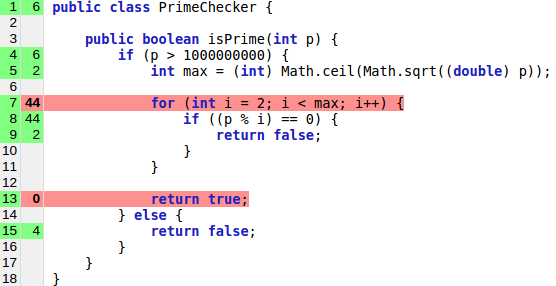
\includegraphics[width=.65\textwidth]{CoverageAnalysis/PrimeChecker.png}
    \caption{Representative of uncovered branches in PrimeChecker.}
    \label{fig:PrimeCheckerAnalysis}
    \vspace{.5cm} 
\end{minipage}
\end{figure}

It seems that part of the code shown in Figure \ref{fig:ColourPickerAnalysis} is not covered because of the influence of a random number.
Test input has no influence on how this random number behaves.
Therefore, EvoSuite cannot generate an input that satisfies the condition to cover that branch. 

\begin{figure}
\centering
\begin{minipage}[c]{\textwidth}
        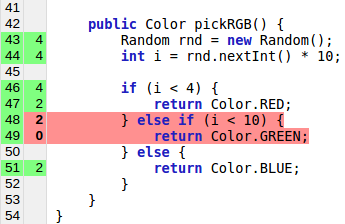
\includegraphics[width=.4\textwidth]{CoverageAnalysis/ColourPicker.png}
    \caption{Representative of uncovered branches in ColourPicker.}
    \label{fig:ColourPickerAnalysis}
    \vspace{.5cm}
\end{minipage}
\end{figure}

In Figure \ref{fig:EnglishNumberToWordsAnalysis}, the \verb|convert(long number)| function accepts a parameter of type \emph{long}.
EvoSuite fails to generate larger numbers to cover the red highlighted lines.
Surprisingly, EvoSuite does not test the boundaries of the long parameter.
Doing so would have resulted in the coverage of at least one of the uncovered branches.

\begin{figure}
\centering
\begin{minipage}[c]{\textwidth}
        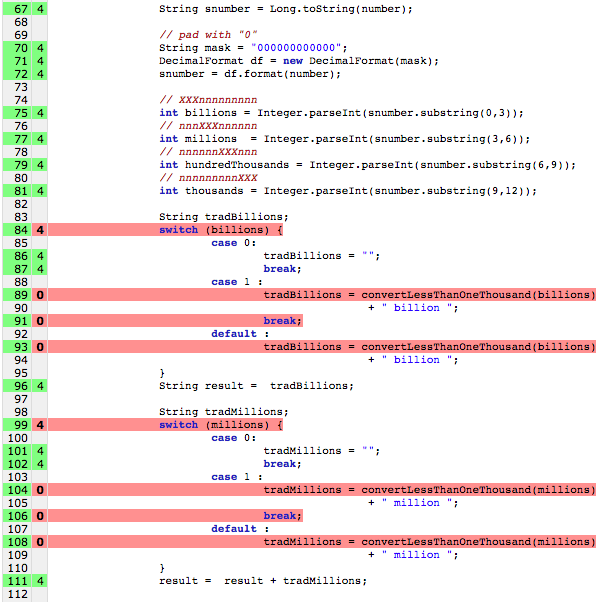
\includegraphics[width=.65\textwidth]{CoverageAnalysis/EnglishNumberToWords.png}
    \caption{Representative of uncovered branches in EnglishNumberToWords.}
    \label{fig:EnglishNumberToWordsAnalysis}
    \vspace{.5cm}
\end{minipage}
\end{figure}


In order to cover the two branches that were not covered by EvoSuite-generated tests in Figure \ref{fig:StringsAnalysis}, a tester would need to input specific strings with a high or low surrogate. 
EvoSuite does not know what high and low surrogate mean and as it does not fall under standard String input, it cannot cover these two branches. 

\begin{figure}
\centering
\begin{minipage}[c]{\textwidth}
        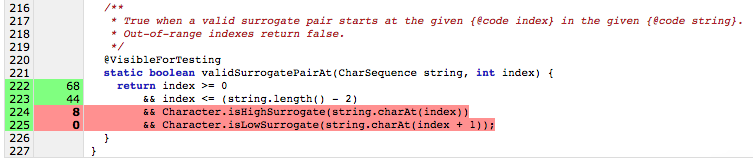
\includegraphics[width=.9\textwidth]{CoverageAnalysis/Strings.png}
    \caption{Representative of uncovered branches in Strings.}
    \label{fig:StringsAnalysis}
    \vspace{.5cm}
\end{minipage}
\end{figure}

In Figure \ref{fig:IntMathAnalysis}, a simple optimization in the case that a left-shift in the power function can be used in not covered.
Since EvoSuite cannot directly reason about the source code, it does not know that such a branch exists and thus there is a possibility that it goes undetected.
This is one of the issues that can arise when using a black-box approach.

\begin{figure}
\centering
\begin{minipage}[c]{\textwidth}
        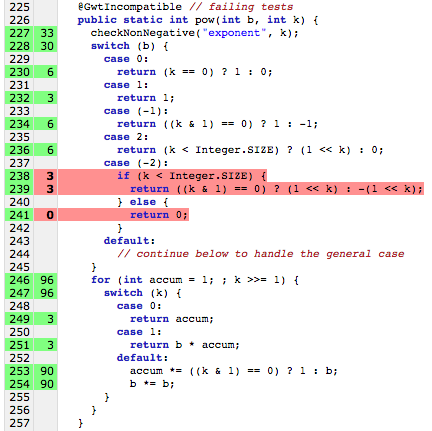
\includegraphics[width=.65\textwidth]{CoverageAnalysis/IntMath.png}
    \caption{Representative of uncovered branches in IntMath.}
    \label{fig:IntMathAnalysis}
    \vspace{.5cm}
\end{minipage}
\end{figure}